%%%%%%%%%%%%%%%%%%%%%%%%%%%%%%%%%%%%%%%%%
% Formal Text-Rich Title Page
% LaTeX Template
% Version 1.0 (27/12/12)
%
% This template has been downloaded from:
% http://www.LaTeXTemplates.com
%
% Original author:
% Peter Wilson (herries.press@earthlink.net)
%
% License:
% CC BY-NC-SA 3.0 (http://creativecommons.org/licenses/by-nc-sa/3.0/)
%
% Instructions for using this template:
% This title page compiles as is. If you wish to include this title page in
% another document, you will need to copy everything before
% \begin{document} into the preamble of your document. The title page is
% then included using \titleGP within your document.
%
%%%%%%%%%%%%%%%%%%%%%%%%%%%%%%%%%%%%%%%%%

%----------------------------------------------------------------------------------------
%	PACKAGES AND OTHER DOCUMENT CONFIGURATIONS
%----------------------------------------------------------------------------------------

\documentclass{article}

\newcommand*{\plogo}{\fbox{$\mathcal{PL}$}} % Generic publisher logo

%----------------------------------------------------------------------------------------
%	TITLE PAGE
%----------------------------------------------------------------------------------------

\newcommand*{\titleGP}{\begingroup % Create the command for including the title page in the document
\centering % Center all text
\vspace*{\baselineskip} % White space at the top of the page

\rule{\textwidth}{1.6pt}\vspace*{-\baselineskip}\vspace*{2pt} % Thick horizontal line
\rule{\textwidth}{0.4pt}\\[\baselineskip] % Thin horizontal line

{\LARGE Prediction Model Selection\\for\\[0.3\baselineskip] \ Bank Telemarketing}\\[0.2\baselineskip] % Title

\rule{\textwidth}{0.4pt}\vspace*{-\baselineskip}\vspace{3.2pt} % Thin horizontal line
\rule{\textwidth}{1.6pt}\\[\baselineskip] % Thick horizontal line

\scshape % Small caps
Report for Statistical Language Programming\\[\baselineskip] % Tagline(s) or further description

\vspace*{2\baselineskip} % Whitespace between location/year and editors

Edited by \\[\baselineskip]
{\Large Yufang,Yan 579027\\Xun,Gong 578553\\ Christoph,Linne \\Emil,Brodersen\par} % Editor list


\vfill % Whitespace between editor names and publisher logo


{\large Humboldt-Universitaet zu Berlin}\par % Publisher

\endgroup}

%----------------------------------------------------------------------------------------
%	BLANK DOCUMENT
%----------------------------------------------------------------------------------------

\usepackage{fancyhdr}
\usepackage{indentfirst}
\usepackage{amsmath}
\usepackage{amssymb}
\usepackage{graphicx}
\usepackage[colorlinks,linkcolor=red]{hyperref}
\usepackage{listings}
\usepackage{natbib}
\usepackage{color}
\definecolor{dkgreen}{rgb}{0,0.6,0}
\definecolor{gray}{rgb}{0.5,0.5,0.5}
\definecolor{mauve}{rgb}{0.58,0,0.82}
\definecolor{lightgray}{gray}{0.95}
\lstset{language=R}
\lstset{breaklines}
\lstset{numbers=left,
	firstnumber = 1,
	backgroundcolor = \color{lightgray},
	numberstyle=\tiny\ttfamily,
	numbersep=5pt,
	numberblanklines=false,
	breaklines=true,
	showstringspaces=false,
	showspaces=false,
	frame=l,
	xleftmargin=5pt,
	xrightmargin=5pt,
	basicstyle=\ttfamily\scriptsize,
	stepnumber=1,
	keywordstyle=\color{black},          
	commentstyle=\color{dkgreen},       
	stringstyle=\color{mauve}         
}
\renewcommand{\lstlistingname}{Code}


\begin{document}
\pagestyle{empty} % Removes page numbers

\titleGP % This command includes the title page

    \newpage
    \pagestyle{fancy}\lhead{Report for Statistical Language Programming}\rhead{Yan,Yufang Xun,Gong\\Christoph,Linne Emil,Brodersen}
    \section{Introduction}
\noindent Nowadays, gigantic amounts of data are available. Therefore, companies in almost all kinds of industries engage in the exploitation of data to obtain competitive advantages over rivals\citep{provost2013data}.\\
The blah technological progress of computers and digitization of businesses makes corporations able to engage directly with customers, collecting and mining information about them, in order to tailor their products in a more optimal way\citep{rust2010rethinking}.\\ 
[\baselineskip]\indent
In particular, in the area of marketing the technologic developments enable a rethinking of marketing strategies by analyzing available data and customer metrics \citep{moro2014data}. \\
This is exactly what this paper will be aiming at. Optimizing the marketing efforts of the company using data mining.\\
In this paper, we focus on optimization models that increase company revenue by offering new products to existing customers. Models for data analysis are more suited for increasing revenue through existing customers than for acquiring new customers, because more information is available on the already existing customers \citep{nobibon2011optimization}. The knowledge of historical data allows the company to implement response models, to predict the probability that a customer will accept the offer of a certain product or service. In the retail banking industry, the banks have access to some of the richest datasets in the world of business \citep{nobibon2011optimization}. This should enable banks to target their marketing efforts towards customers that are more likely to accept the marketed products, which leads to lower marketing costs and increased profit.\\
In this paper, we study data related to a telemarketing campaign by a Portuguese Bank in the period of 2008-2010. Specifically we want to show that the bank can succesfully classify their customers as “accepters” or “decliners” of an offer made through a telemarketing campaign.\\
Several models can do such a classification task. In this paper, we use the Logistic Regression, Decision Trees, Random Forest and Neural Network.
The logistic regression and decision trees have the advantage that they make it easy to interpret which variables affect the classification probability. Random forest and neural network have the advantage that they can model highly complex nonlinear relations which tend to make these two models more accurate compared to the logistic regression and decision trees. However, due to the complexity of these models they are difficult to interpret and understand.\\
We fit all four models, and by using the AUC measure we conclude on which model does the most accurate predictions.
\\
    \newpage
    \pagestyle{fancy}\lhead{Report for Statistical Language Programming}\rhead{Yan,Yufang Christoph,Linne\\Xun,Gong Emil,Brodersen}
    \section{Theory and Design}
    \subsection{Data pre-processing}
	\subsubsection{Data Cleaning and Imputing}
	\noindent Multiple imputation\citep{DB1987multiple} is the method of choice for complex incomplete data problems. There are two methods for imputing multivariate data: one is joint modeling (JM) and the other one fully conditional specification (FCS)\citep{stef2007multiple}. \\
	[\baselineskip]\indent JM imputation\citep{JL1997analysis} requires the specification of a parametric joint model 
	$P\left({x}^{mis}|{x}^{obs},\theta\right)$ for the complete data and a prior distribution $P(\theta)$  for parameter  $\theta$. Imputations are independent draws from the posterior predictive distribution of the missing data given the observed data $P \left(x|\theta\right)$ , which under the ignorability assumption: \\
	\begin{equation}\label{}
		P({x}^{mis},{x}^{obs})=
		\int P\left({x}^{mis}|{x}^{obs},\theta\right)p\left(\theta| {x}^{obs}\right)\, \mathrm{d}x\\
	\end{equation}
	\\
	[\baselineskip]\indent FCS \citep{stef2015mice} specifies the multivariate imputation model on a variable-by-variable basis by a set of conditional densities, one for each incomplete variable. Multivariate Imputation by Chained Equations (MICE) is on the basis of FCS:\\
	\begin{eqnarray}\label{}
		\begin{split}
			&\psi_1^{(t)}\sim p(\psi_1)p\left( x_1^{obs}|x_2^{(t-1)},x_3^{(t-1)},\dots,\dots,x_{R}^{(t-1)}, x_{R+1},\dots, x_K, \psi_1\right)\\
			&x_1^{mis(t)}\sim p\left(x_1^{mis}|x_2^{(t-1)},x_3^{(t-1)},\dots,\dots,x_{R}^{(t-1)}, x_{R+1},\dots, x_K, \psi_1^{(t)}\right)\\
			&\psi_2^{(t)}\sim p(\psi_2)p\left( x_2^{obs}|x_1^{(t)},x_3^{(t-1)},\dots,\dots,x_{R}^{(t-1)}, x_{R+1},\dots, x_K, \psi_2\right)\\
			&x_2^{mis(t)}\sim p\left(x_2^{mis}|x_1^{(t)},x_3^{(t-1)},\dots,x_R^{(t-1)},x_{R+1},\dots, x_K, \psi_2^{(t)}\right)\\
			& \vdots\\
			&\psi_R^{(t)}\sim p(\psi_R)p\left( x_R^{obs}|x_1^{(t)},x_2^{(t)},\dots,x_{R-1}^{(t)}, x_{R+1},\dots, x_K, \psi_R\right)\\
			&x_R^{mis(t)}\sim p\left(x_ R^{mis}|x_1^{(t)},x_2^{(t)},\dots,x_{R-1}^{(t)}, x_{R+1},\dots, x_K, \psi_ R^{(t)}\right)
		\end{split}
	\end{eqnarray}
	\\

	\subsubsection{Imbalanced data resampling}
	\noindent A dataset is imbalanced if the classes are not approximately equally represented. Imbalanced
	data sets exists in many real-world domains, such as telecommunications management, detection of fraudulent telephone, detection of oil spills in satellite images and so on. In these domains, what we are really interested in is the minority class other than the majority class. Thus, we need a fairly high prediction for the minority class. \\
	[\baselineskip]\noindent There are two main ways addressed the issue of class imbalance.	One is cost sensitive learning, the other is to re-sample the original dataset. Here we introduce an approach, SMOTE(Synthetic Minority Class Oversampling), which blends under-sampling of the majority class with a special form of over-sampling the minority class.\citep{smote}
	 \begin{itemize}
		\item For each minority class \boldmath$ x_{i} $
			\begin{itemize}
		 	\item Identify K nearest neighbors of minority class
		 	\item Randomly select one of these neighbors \boldmath$ x_{ij} $
		 	\begin{itemize}
		 	\item Calculate feature vector difference
		 	\item Multiply with random number $\delta \in$ [0,1]
		 	\item Add result to \boldmath$ x_{i} $
		 	\end{itemize}
			\item Generate a new point between $ x_{i} $ and $x_{ij} $\\
     \begin{equation}\label{}
x_{new} =  x_{i} + (x_{i}-x_{ij})*\delta \\
    \end{equation}
		\end{itemize}
		\item For the majority class, under-sampled by randomly removing samples from the majority class
		population until the minority class becomes some specified percentage of the majority class.
	\end{itemize}
	 
    \subsection{Prediction Models} 
      \subsubsection{Logit Regression Model}
      \noindent General linear model (GLM) \citep{p1982generalized} usually refers to conventional linear regression models for a continuous response variable given continuous and/or categorical predictors. In logistic regression, probability of the response taking a particular value is modeled based on combination of values taken by the predictors. The form is $ y_i\sim N(x_i^T\beta,\alpha^2)$, where $x_i$ contains known covariates and $\beta$ contains the coefficients to be estimated. These models are fit by least squares and weighted least squares. In these models, the response variable $y_i$ is assumed to follow an exponential family distribution with mean $\mu_i$, which is assumed to be some (often nonlinear) function of $x_i^T\beta$. Some would call these “nonlinear” because  $\mu_i$ is often a nonlinear function of the covariates, but McCullagh and Nelder\citep{p1982generalized} consider them to be linear, because the covariates affect the distribution of $y_i$ only through the linear combination $x_i^T\beta$. \\
      [\baselineskip]\indent Binary Logistic Regression models how binary response variable $Y$ depends on a set of $k$ explanatory variables, $X=(X_1, X_2,\dots, X_k)$.\\
      \begin{equation}\label{}
      	Logit(\pi)=log(\frac{\pi}{1-{\pi}})=
      	\beta_0+\beta{x_1}+\dots+
      	\beta{x_{k'}}\\
      \end{equation}
      which models the log odds of probability of "success" as a function of explanatory variables. In $(3)$, the distribution of $Y$ is assumed to be Binomial $(n,\pi)$, where $\pi $ is a probability of "success". $X$'s are explanatory variables (can be continuous, discrete, or both) and are linear in the parameters, e.g., $\beta_0 + \beta_{x_i} \dots +\beta_{x_k}$. Transformation of the X's themselves are allowed like in linear regression; this holds for any GLM. The Logit Link($ Logit(\pi)=log(\frac{\pi}{1-{\pi}})$) models the log odds of the mean, and the mean here is $\pi$. Binary logistic regression models are also known as logit models when the predictors are all categorical \citep{p1982generalized} .\\
    
    	\subsubsection{Decision Tree Model}
            \noindent Decision tree induction algorithms have long been popular in machine learning, statistics, and other disciplines for solving classification and related tasks. Decision Tree models where the target variable is a factor are called classification trees. In the classification tree structures, leaves represent class labels and branches represent conjunctions of features that lead to those class labels. Each node represent an splitting rule based on the value of one specific input variable, which is calculated by recursive partitioning. The recursion is completed when splitting no longer adds value to the predictions. This process of top-down induction of decision trees (TDIDT) \citep{quinlan} is an example of a greedy algorithm.
    	\subsubsection{Random Forest Model}
    	\subsubsection{Neural Network Model}
    	\noindent Neural Network models are mathematical models that are, loosely put, based on how the biological brain works \citep{baesens2003using}. This allows for highly complex nonlinear relationships between the input and the predicted variables. 
    	A neural network is a system of neurons. Each individual neuron is simple. It receives an input, process it and generates an output. Though each neuron is by itself simple, a network of neurons can produce very complex and intelligent calculations \citep{shiffman2012nature}. 
    	A neural network typically consists of three layers. An input layer, a hidden layer and an output layer. The need for only three layers is known as the universal approximation theorem and states that a neural network with three layers can approximate any continuous function to arbitrary degrees of accuracy \citep{hornik1989multilayer}.
    \subsection{Model Performance Evaluation}
    \noindent A class can be assigned from a probabilistic outcome by assigning a threshold $D$, such that event $c$ is true if $P\left(c| x_k\right)>D$. The receiver operating characteristic (ROC) curve shows the performance of a two class classifier across the range of possible threshold (D) values, plotting one minus the specificity versus the sensitivity\citep{tom2006an}. The overall accuracy is given by the area under the curve ($AUC = \int_0^1ROC \mathrm{d}D$), measuring the degree of discrimination that can be obtained from a given model. AUC is a classification index\citep{david2011performance} that presents advantages of being independent of the class frequency or specific false positive/negative costs. The ideal method should present an AUC of 1.0, while an AUC of 0.5 denotes a random classifier.
    
    
    
    \newpage
    \pagestyle{fancy}\lhead{Report for Statistical Language Programming}\rhead{Yan,Yufang Christoph,Linne\\Xun,Gong Emil,Brodersen}
    \section{Implementation}
    \subsection{Data Pre-processing}
    \subsubsection{Data Imputation}
    \noindent Codes for cleaning and imputing data consists of two parts: first one is used to detect the pattern of missing data, in order to choose the right algorithm to impute the incomplete data. \\
    \begin{lstlisting}
mice_plot<-aggr(data_missing,col=c('navyblue','yellow'),numbers=TRUE,sortVars=TRUE,labels=names(data_missing),cex.axis=.7,gap=3,ylab=c("Missing_Data_Ratio","Missing_Data_Pattern"))
    \end{lstlisting}
    In line 1 above, the report used aggr() function provided by MICE package. The function yielded one histogram and one graph, which were named "Missing Data Ratio" and  "Missing Data Pattern" respectively. In the graph, variables without missing value was marked with color navy blue, and incomplete variables were marked with color yellow. Variables were sorted according to the severity of missing.\\
     \begin{lstlisting}
tempData <- mice(data_missing,m=5,maxit=10,meth,seed=500,diagnostics=T)
data_complete <- complete(tempData,1)
    \end{lstlisting}
     In line 1 above, based on the pattern of missing value, the report imputes missing value. $"tempData"$ contains complete datasets imputed by mice() function. $"m"$ denotes how many sets of complete dataset imputed and $"meth"$ denotes which method is used. $"maxit"$ means how many iterations are needed, in which normally 10 is good enough. $"diagnostics"$ is used to evaluate how good the imputation is. Codes in line 2 chooses the first dataset from m datasets created by line 1. \\   
     \subsubsection{Data Balancing}
	 \noindent Core part of the code for data balancing
     \begin{lstlisting}
library(unbalanced)
library(FNN)
# Calculate the SMOTE resamping scale parameters
sum = length(data_train$y)
ori_min = length(which(data_train$y == 1))
new_min = round(sum*(1/2)) - ori_min
over_s = (round(sum*(1/2)) / ori_min) - 1 
un_s = (sum - all_min)/new_min 
newdata= ubSMOTE(X,Y, k = 5,
		perc.over = 100*over_s,
		perc.under = 100*un_s,
		verbose = FALSE)
     \end{lstlisting}
     Above codes shows how we implement the SMOTE algorithm using the package "unbalanced". From line 4 to 7, function ubSMOTE() is called. First we specify the input variables X and response variable Y from the imbalanced dataset. The parameter K defines the numbers of nearst neighbors which are randomly choose. The scaling parameter per.over and perc.under control the amount of over-sampling of the minority class and under-sampling of the majority classes, respectively. For instance, if per.over = 200, per.under = 100, it means $200/100 = 2$ new minority samples will be generated for each minority sample. And at the same time, $100/100 *2 = 2 $ majority samples will be randomly chosen from the majority samples. 
    \subsection{Prediction Models}
    \noindent The core codes in this part divides into two part, one is settings for prediction model,the other one is prediction model: 
   \begin{lstlisting}
cvCtrl <- trainControl(method="cv",number,classProbs=TRUE,summaryFunction=twoClassSummary,verboseIter=TRUE)
predict_model <- train(y ~ .,data,method,family,trControl=cvCtrl, metric="ROC",tuneLength)
    \end{lstlisting}
    \indent The report uses caret package to train predict models. The codes in line 1 makes the settings for the train() function:$method$ is cross validation. It means when training the model, the function will randomly choose one part of data as testing data, and test the model trained based on the train data. In this way, the model is improved. $number$ is the number of folds in cross validation. If the chosen number is n, then $n-1$ folds are used to train the prediction model and the left one is to test whether the model is good enough.  $classProbs$ means whether class probabilities be computed for classification models (along with predicted values) in each resample. Since the purpose of the report is to predict whether a customer will or not buy a product, $True$ is chosen in this report. Similarly, $twoClassSummary$ is also chosen to compute performance metrics across resamples. $verboseIter$ is also chosen for printing a training log.\\
    [\baselineskip]\indent In line 2, specific models are trained in train() function. The target variable is $y$, $"."$ represents all other variables in the data as predictors. The $method$ is the most important part of the codes. There are several options and the report uses $"glm"$ (generalized linear model) and $"nnet"$ (neural network). $trControl$ is set in Line 1. $metric$ is the method used for evaluate whether the model is good or not. $tuneLegth$ denotes the amount of granularity in the tuning parameter grid.  \\
    \subsubsection{Decision Tree Model}
    \noindent Core part of the code for building the decision tree
    \begin{lstlisting}
library(rpart)
# pre-pruning the tree
rpart.control= rpart.control(minsplit=5, 
	minbucket = round(5/3),
	maxdepth=4, 
	cp=0.001)
   
# build the model
tree <- rpart(y~.,data = train,
		method = "class", 
	   	parms=list(split="Gini/Information"), 
	   	control = rpart.control)

# prediction
prediction <- predict(tree ,newdata = test, type = "prob")
    
    \end{lstlisting}

     \noindent We use the package rpart, which implement the popular non-parametric CART algorithm. \\
     [\baselineskip]\noindent Parameters defined in line 3 is to pre-prune the tree in case the tree grows to large. We set three stopping criterions. The minsplit parameter is the smallest number of observations in the parent node that could be split further. The parameter minbucket provides the smallest number of observations that are allowed in a terminal node. And maxdepth parameter defined a certain depth of the tree from root to leafs. \\
     [\baselineskip]\noindent From line 6 to 9, we build the decision tree model using function rpart(). As we are building a classification tree, so we choose the parameter method = "class". The parameter parms defines the splitting function. The splitting index can be "Gini" or "Information", which are two functions to calculate the Impurity of each node. “Gini” will tend to find the largest class, and “Information” \begin{flushleft}
     
     \end{flushleft}tends to find groups of classes that make up ~50\% of the data.(detail calculation and equation in \citep{terry})\\
     [\baselineskip]\noindent In line 12, the predict function will return the probability of each classes as we define the parameter type = "prob".
     
     \subsubsection{Neural Network Model}
        \noindent The neural network can be trained in three different ways; supervised learning, unsupervised learning and reinforcement learning. Supervised learning can be used when one already has a dataset containing the answers to the question that we want to predict, and this is the training method that will be used in this paper.\\
     The model attempts to predict outcomes, initiating this procedure with random weights. The errors of the predicted outcomes are then calculated and fed backwards through the model and used to update the weights. Through this process, the weights of the network are updated in such a way that the neurons recognise different patterns of the input space. This process continues until the weights have been optimally set or a maximum number of iterations have been reached. This process is called ‘backward propagation’. Backward propagation requires that the activation functions are differentiable. The standard approach is to use a sigmoid function such as a logit regression.\\
     [\baselineskip]\indent To train the neural network model in R, we make use of the 'caret' package. We first use the 'trainControl' function to specify the options of the neural network algorithm.:
     \begin{lstlisting}
model.control<- trainControl(
method = "cv", # 'cv' for cross validation
number = 5, # number of folds in cross validation
classProbs = TRUE, # Calculate class probabilities in each resample
summaryFunction = twoClassSummary, # Compute sensitivity, specificity and AUC for each resample
returnData = FALSE # The training data will not be included in the ouput training object
     )
     \end{lstlisting}
     \indent In line 2 we specify that we would like to train the model using cross validation, and in line 3 we specify how many folds we would like to use in the cross validation. By choosing five folds, we divide the data into 5 equally large subsets and leave one of them out. This is repeated for all five subsets. Line 4 and 5 specify that we would like to calculate class probabilities and sensitivity/specificity and AUC for all resamples. Line 6 specifies that we are not interested in saving the training data.\\
     Next, we consider the parameters for the neural network.
     \begin{lstlisting}
nn.parms <- expand.grid(decay = c(0, 10^seq(-3, 0, 1)), size = seq(3,15,1))
     \end{lstlisting}
     
     To choose the optimal parameters for our neural network, we define a grid of parameters that we would like to test. As previously described, the neural network needs two parameters to be specified, namely weight decay and number of nodes in the hidden layer. To choose the optimal values of the parameters, we use the function 'expand.grid' to specify a grid within which to search for optimal parameters. We specify that we would like to search for a weight decay of (0,001; 0,01; 0,1; 1) and a number of hidden nodes between three and fifteen. \\
     [\baselineskip]\indent After having specified the options and the parameters we want to test, we initiate the training of the neural network.
     \begin{lstlisting}
nn <- train(y~., data = train,  
method = "nnet", 
maxit = 500, 
trace = FALSE, # options for nnet function
tuneGrid = nn.parms, # parameters to be tested
metric = "ROC", trControl = model.control)
     \end{lstlisting}
     In line 1 we specify that the variable we want to predict is 'y' and that we want to use all variables as explanatory variables. In line 5 we give the grid that we want to search for optimal parameters. In line 6 we give the options that we specified previously.
     \\
     \subsection{Model Performance Evaluation}
     \noindent Codes in line 3 predict make the prediction with the model trained in line 2. $type$, containing "raw" and "prob", defines the output is class predictions or class probabilities. Line 3 outputs class prediction and line 5 class probability. Codes in line 4 compares this prediction with the real behavior of customers. Since the report hopes to predict customer who buys the product, "Yes" is chosen in line 4. In line 5 to 8, ROC curve is calculated based on the confusion matrix.\\
     \begin{lstlisting}
prediction1 <- predict.train(model,newdata)
confusionMatrix(prediction,data$y, positive="yes")
prediction2 <- predict(model, type = "prob")[,2]
roc<-roc(data$y,prediction2)
auc(roc)
plot.roc(roc)
     \end{lstlisting}
     
     
    \newpage
    \pagestyle{fancy}\lhead{Report for Statistical Language Programming}\rhead{Yan,Yufang Christoph,Linne\\Xun,Gong Emil,Brodersen}
    \section{Empirical Study/Testing}
    \subsection{Data Input and Description}
    \noindent The report used dataset from \url{http://archive.ics.uci.edu/ml/datasets/Bank+Marketing}. The data is related with direct marketing campaigns of a Portuguese banking institution. The time period is May 2008-Nov 2010 and the dataset contains 41188 respondents. The marketing campaigns were based on phone calls, in order to access if the product (bank term deposit) would be ("yes") or not ("no") subscribed(the target variable is "y"). The predictor variables with  are listed below in table 1:\\
    \begin{center}
	\begin{table}[!hbp] \centering \label{}  
		\begin{tabular}{ccc} 
			\hline\hline \\[-1.8ex] 
			{Demographic Info}  & {Marketing Info} & {Macroeconomy Info} 
			\\ 
			\hline \\[-1.8ex] 
			age (numeric) & contact(categorical) & emp.yar.rate(numeric)
			\\ 
			job(categrical) & month(categorical) & cons.price.idx(numeric)
			\\ 
			marital(categorical) & day.of.week(categorical) & cons.conf.idx(numeric)
			\\ 
			education(categorical) & duration(numeric) & euribor3m(numeric)
			\\ 
			default(categrical) & campain(numeric) & nr.employed(numeric)
			\\ 
			housing(categorical) & pdays(numeric)
			\\ 
			loan(categorical) & previous(numeric) 
			\\ 
			 & poutcome(categorical) 
			\\ 
			\hline\hline 
		\end{tabular} 
		\caption{Predictor Variables}
    	\end{table}
        \end{center}
        Variables "default" and “duration" are not included in the final analysis. There are only three respondents had default records, which led to exclusion of "default" due to very low variance \citep{max2016applied}. Variable "duration" describes last contact duration. However, this attribute highly affects the output target (e.g., if duration=0 then y="no"). Yet, the duration is not known before a call is performed. Also, after the end of the call "y" is obviously known. Thus, this input is discarded if the intention is to have a realistic predictive model.\\               
         \subsection{Data Pre-processing}    
         \subsubsection{Missing Value Pattern Overview}    
          \begin{itemize}
         	\item \textbf{Function}
         \end{itemize}
         \begin{lstlisting}
mice_plot <- aggr(bank, col=c('navyblue','yellow'), numbers=TRUE, sortVars=TRUE, labels=names(bank), cex.axis=.7, gap=3, ylab=c("Missing_Data_Ratio", "Missing_Data_Pattern"))
         \end{lstlisting}
         \begin{itemize}
         	\item \textbf{Expected Output}
         \end{itemize}
         The report expects an overview of missing value, both its ratio and pattern, based on which an appropriate imputation method is chosen. The aggr() function from MICE package will yield two graph, one is a histogram showing the ratio of missing value in every variable, the other one is a graph showing missing values according to observations, i.e., the pattern of missing data.\\
         \begin{itemize}
         	\item \textbf{Actual Output}
         \end{itemize}
      \noindent The Figure 1 indicates missing value pattern of this dataset. On the left side of Figure 1 is the ratio of missing value of each variable. Specifically, variable "education" has more than $4\%$ respondents without educational information. Other variables with missing values are "housing", "loan", "job" and "marital". The missing value ratio of those five variables are all under $10\%$, which is acceptable in a statistical analysis perspective. On the right side of Figure 1 is missing value pattern from the perspective of observations: the bottom row of graph, with all cubic in color blue, represents 38245 cases with complete data. The row above, with one cubic in yellow and others in blue, represents 1558 observations with educational information missing and other information complete. For the same reason, the third row from the bottom indicates 946 observations with both housing and loan information missing. In a word, the cubic in yellow shows the how the data is missing. \\
         \begin{figure}[htbp] 
         \centering
         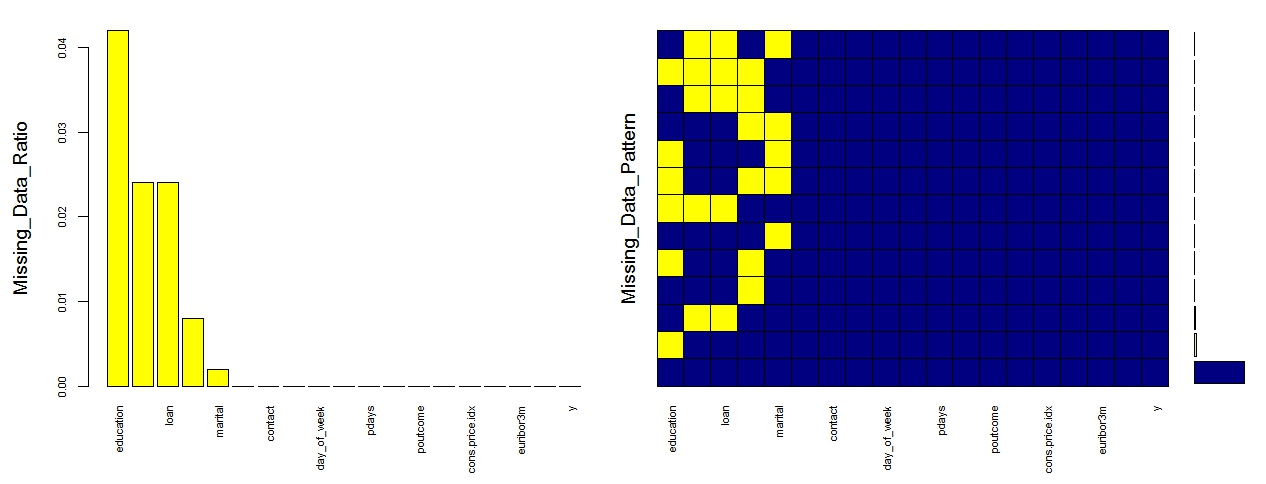
\includegraphics[width=5.5in]{MVP.jpeg} 
         \caption{Missing Value Ratio and Pattern}\label{fig:1} 
        \end{figure}
         \begin{itemize}
         	\item \textbf{Comments}
         \end{itemize}
        \noindent According to the pattern showed in Figure 1,the missing value is missing at random(MAR). Therefore, the report decides to impute the missing value with MICE package in the next section.\\
         \subsubsection{Data Imputation}
         \begin{itemize}
         	\item \textbf{Function}
         \end{itemize}
         \begin{lstlisting}
# Data Preparation
n <- nrow(bank) 
sample.size <- ceiling(n*0.8) 
idx.train <- sample(n, sample.size) 
bank_train <- bank[idx.train, ] 
bank_test <-  bank[-idx.train, ]         
# Data Imputing for Train and Test Dataset
tempData1 <- mice(bank_train,m=5,maxit=10,meth="polyreg",seed=500,diagnostics=T)
bankclean_train <- complete(tempData1,1)
tempData2 <- mice(bank_test,m=5,maxit=10,meth="polyreg",seed=500,diagnostics=T)
pred <- tempData2$predictorMatrix
pred[,"y"] <- 0
tempData3 <- mice(bank_test, pred=pred, pri=F)
bankclean_test <- complete(tempData3,1)
         \end{lstlisting}
         \begin{itemize}
         	\item \textbf{Input Description}
         \end{itemize}
     \noindent Because the purpose of the report is to make precise prediction of "y", so predictor variables cannot be affected by the target variable. However, the imputation process is in essence predictions made based on other available variables. Therefore, in test dataset, missing values are predicted only by other predictor variables, while in train dataset, it is allowed to be predicted by all variables including target variable.As a result, before imputing missing value, the report splits the whole dataset into train data set($80\%$) and test data set($20\%$). Line 1 to 6 achieved this goal. So far, the dataset $"bank"$, which is originally input, is split into $"bank\_train"$ and $"bank\_test"$. \\
     [\baselineskip]\indent Then both incomplete datasets were completed with MICE package function in line 7 to 16. In line 10, there are five sets of predictions are created by mice function, and line 9 indicates the report picks the first set as the basis for further analysis. The same also goes for test dataset, with the exception that target variable "y" is excluded. In line 12 and 13, the report removes "y" as a predictor for missing values in test dataset. So far, both train and test data are free from missing value, and are renamed as $"bankclean\_train"$ and $"bankclean\_test"$.\\           
         \begin{itemize}
         	\item \textbf{Expected Output}
         \end{itemize}
         The report expects that all missing values of each variable are correctly and precisely predicted to the best extent. \\
         \begin{itemize}
         	\item \textbf{Actual Output}
         \end{itemize}
          Train dataset and test dataset are free of missing value after imputation. Therefore, both of datasets are prepared for further analysis. \\
         \begin{itemize}
         	\item \textbf{Comments}
         \end{itemize}
     \noindent As showed in table 1, even though some variables(for example macro economy index) are in numeric format, they can also be regarded as categorical variables since each of factor contains less than ten levels. Therefore, the imputation process deals with all variables as categorical variables and chooses "polyreg" as imputing method. Unfortunately, "polyreg" makes it more difficult to evaluate the imputation quality, since existing functions provided by MICE is for numeric variables.\\
       \subsubsection{Data Balancing}
       \begin{itemize}
       	\item \textbf{Function}
       \end{itemize}
\begin{lstlisting}
# Adjust the response variable to 0/1 factor
data_train$y=as.factor(ifelse(data_train$y=="yes","1","0"))

# Resampling
newdata = ubSMOTE(data_train[,-20],data_train[,20], 
		k = 10, 
		perc.over = 100*over_s, 
		perc.under = 100*un_s,
		verbose = FALSE)
\end{lstlisting}
\begin{itemize}
	\item \textbf{Input Description}
\end{itemize}
   		\begin{itemize}
   		\item \textbf{Expected Output}
   		We will get the balanced traininng set with approximately 50\% of positive response samples. And the prediction is assumed to be improved with the model trained by balanced data.  
   		\end{itemize}
   	   	\begin{itemize}
   		\item \textbf{Actual Output}
   		\end{itemize}
   	  \begin{center}
   		\begin{table}[!htbp]
   			\centering  
   			\begin{tabular}{llc}
   				\hline
   				\hline\\[-1.8ex]

   				 & Imbalanced Data & Balanced Data \\
   				\hline \\[-1.8ex] 
   				No &  29270 & 14223  \\ 
   				\hline \\[-1.8ex] 
   				Yes&  3681 & 14724 \\ 
   				\hline
   				\hline
   			\end{tabular}  
   			\caption{Data balancing comparison} 
   		\end{table}
   	\end{center}
   	   	\begin{itemize}
		\item \textbf{Comments}
		\end{itemize}
       \subsection{Building Prediction Models}
       \subsubsection{Logit Regression Model}
       \begin{itemize}
     	\item \textbf{Function}
       \end{itemize}
       \begin{lstlisting}
# Data Preparation
bank.train.dummy <- predict(dummyVars(y ~ .,data=balancedTrain), newdata=balancedTrain)
bank.train.dummy <- data.frame(bank.train.dummy, y=factor(balancedTrain$y))
bank.test.dummy <- predict(dummyVars(y ~ . ,data=bankclean_test), newdata=bankclean_test)
bank.test.dummy <- data.frame(bank.test.dummy, y=factor(bankclean_test$y))
# Logit Regression Model
logit <- train(y ~ ., data=bank.train.dummy, method="glm", family = binomial("logit"), preProc = c("center", "scale"), trControl=trainControl(method="cv", classProbs=TRUE, summaryFunction=twoClassSummary, verboseIter=TRUE), metric="ROC",tuneLength=1)
# Evaluation
bank.test.class <- subset(bank.test.dummy, select=c(y), drop=TRUE)
predict.logit.test1<-predict.train(logit,bank.test.dummy)
confusionMatrix(predict.logit.test1, bank.test.class, positive="yes") 
predict.logit.test2 <- predict(logit, bank.test.dummy, type="prob")[,2]
logit.test.roc<-roc(bank.test.dummy$y,predict.logit.test2)
auc(logit.test.roc)
plot.roc(logit.test.roc)
       \end{lstlisting}
       \begin{itemize}
       \item \textbf{Input Description}
       \end{itemize}
       \noindent The logit regression model requires all factor variables, i.e., categorical variables, need to be changed into dummy variables. As the function above shows, all factor variables are changed by dummyVars function. As a result, there are 55 variables in the new dataset $"bank.train.dummy"$. The test dataset is also transformed with the same code. \\
       [\baselineskip]\indent To implement logit regression modeling, the report adopts train function provided by caret package in R, then specifies the method as $"glm"$ and family as $"binomial"("logit")$. Cross validation is chosen to improve model accuracy. Meanwhile, the dataset is requited to be standardized before logistic analysis, which is also achieved within the train function. \\
       [\baselineskip]\indent After the model is derived, it is evaluated by comparing its prediction with real customer behavior. \\
       \begin{itemize}
       	\item \textbf{Expected Output}
       \end{itemize}
   A binary logit analysis is expected to yield the relationship between each predictor variable and the target variable, considering other predictor variables hold still. Additionally, comparing predicted result with real result, the report also expect to evaluate how good the model is. An AUC index and an ROC curve are also expected to evaluate how well the logistic model works with future data.\\   
\begin{itemize}
	\item \textbf{Actual Output}
\end{itemize}
  \noindent The equation from binary logistic regression model is showed below in equation (4). Comparing coefficients of each predictor, it is obvious that macro economy situation is significantly important issue when customers considering purchasing bank product. Customer demographic information is relatively less important(most coefficients are less than 0.1). The marketing strategies of bank is of importance. Specifically, the marketing conducted via cellphone is more useful than cellular, and Wednesday is the best time to make marketing calls. Customers who rejected in last marketing campaign is more likely to reject again. \\
  \begin{eqnarray}\label{}
  \begin{split}
  y =& 0.21-0.06\ast{age}-0.10\ast{job.bluecollar}+0.05\ast{job.retired}+0.07\ast{job.student}\\
  - &0.16\ast{marital.married}-0.04\ast{education.basic4y}-0.03\ast{education.basic9y}\\
  - &0.04\ast{education.highschool}-0.05\ast{education.professionalcours}\\
  + &0.08\ast{housing.no}-0.52\ast{loan.no}-0.10\ast{contact.cellular}+0.10\ast{month.aug}\\
  + &0.18\ast{month.jul}+0.21\ast{month.mar}-0.31\ast{month.may}-0.09\ast{month.nov}\\
  + &0.06\ast{month.oct}-0.05\ast{day\_of\_weekfri}-0.12\ast{day\_of\_weekmon}\\
  - &0.04\ast{day\_of\_weekthu}-0.04\ast{day_of_weektue}-0.10\ast{campaign}+0.34\ast{pdays}\\
  - &0.16\ast{poutcome.nonexistent}-1.36\ast{emp.var.rate}+ 0.48\ast{cons.price.idx} \\
  + &0.07\ast{cons.conf.idx}+0.70\ast{euribor3m}+-0.65\ast{nr.employed}
  \end{split}
  \end{eqnarray}
How good is the derived model? The matrix in table 2 compares the prediction made by the model with real customer behavior: in train dataset, of 14724 customers who actually deposited, the model predicts 10605 ones correctly, while it predicts 4119 are potential customers while the fact is opposite. Meanwhile, the model predicts 2624 customers will buy the product while they actually did not. In test dataset, the model predict 6506 cases correctly(624 customers who says yes, and 5882 customers says no). Based on the confusion matrix, ROC curve in Figure 2 is created to evaluate the model visually. \\
  \begin{center}
  	\begin{table}[!htbp]
  		\centering  
\begin{tabular}{llc}
	\hline
	\hline\\[-1.8ex]
	& \multicolumn{2}{c}{Reference(Traindata/Testdata)} \\
	\cline{2-3}\\[-1.8ex]
	Prediction & No & Yes \\
	\hline \\[-1.8ex] 
	No & 11599/5882 &4119/335 \\ 
	\hline \\[-1.8ex] 
	Yes& 2624/1396 &10605/624\\ 
	\hline
	\hline
\end{tabular}  
\caption{Confusion Matrix of Logit Model} 
\end{table}
\end{center}

\begin{itemize}
	\item \textbf{Comments}
\end{itemize}
\noindent An index of AUC can be calculated from ROC curve. The AUC of prediction on train dataset equals to 0.8286 and on test dataset is 0.7769. Figure 2 shows the ROC curve of model performance on test dataset. \\
	\subsubsection{Decision Tree Model}
	 \begin{itemize}
		\item \textbf{Function}
	\end{itemize}
	
	\begin{lstlisting}
# pre-pruning the tree in case of overfitting
rpart.control= rpart.control(minsplit=5, minbucket = round(5/3), maxdepth=4, cp=0.001)
# decision tree model
dtm<-rpart(y~.,data=balancedTrain,parms=list(split="information"),  control=rpart.control)
# plot the decision tree model
rpart.plot(dtm,type=1, extra=104,
cex = 0.55, fallen.leaves= FALSE, faclen = 3)
# test the classifier in testing dataset
pred_dtm <- predict(dtm,newdata=data_test,type = "prob")
# set the threshold to see the Confusion Matrix
threshold <- 0.5
pred_class<-as.matrix(factor(ifelse(pred_dtm[,2]>threshold,"yes","no")))
confusionMatrix(pred_class, data_test$y,positive = "yes")
	\end{lstlisting}
	\begin{itemize}
	\item \textbf{Input Description}
	\end{itemize}
	\indent Here we are building a classification tree as our response variable y is a factor. Since the decision tree can deal with both numerical and categorical variables, we can directly input the balanced training set. We choose to use "information" as splitting criteria, as most of the input variables are categorical variables. \\
	[\baselineskip]\noindent After the model is trained, we will test it based on our testing set. And evaluate the prediction performance by calculating the confusion matrix with 0.5 threshold.
	
	 \begin{itemize}
		\item \textbf{Expected Output}
	 \end{itemize}
 	 \indent As a result of model building,we will get an well-shaped binary tree decision algorithm, which is displayed as a flowchart like tree, where each split represent a "Yes/No" decision. For the prediction test, we will expect an accuracy than better 0,5.
 
	 \begin{itemize}
 		\item \textbf{Actual Output}
		\begin{figure}
			\centering
			\includegraphics
			[width=1\linewidth]
%[scale=0.5]
			{DT_output}
			\caption{}
			\label{fig:104adjdt}
		\end{figure}
		\begin{center}
			\begin{table}[!htbp]
				\centering  
				\begin{tabular}{llc}
					\hline
					\hline\\[-1.8ex]
					& \multicolumn{2}{c}{Reference(Traindata/Testdata)} \\
					\cline{2-3}\\[-1.8ex]
					Prediction & No & Yes \\
					\hline \\[-1.8ex] 
					No & 6572\textcolor{red}{(0.9)} &454 \\ 
					\hline \\[-1.8ex] 
					Yes& 706 &505 \textcolor{red}{(0.53)} \\ 
					\hline
					\hline
				\end{tabular} 
				\caption{Confusion Matrix of Decision Tree Model} 
			\end{table}
		\end{center}
 	 \end{itemize}
  	 \begin{itemize}
  		\item \textbf{Comments}
  	\end{itemize}
  		\noindent As we can see in Figure 2, the trained decision tree model grows pretty good. We can easily interpret the classification rules from it. For example, the variable at the root is social economic variable, euribor3m, which represent the most import explanatory variables for classification. We can say that, in our training model, if the euribor3m index is smaller than 4.9 and cons.price.idx is bigger than 93, which 24\% of the samples fall into, the probability of a successful call is 0.95.\\
  		[\baselineskip]\noindent From the confusion matrix showed in Table 3, we can evaluate the prediction performance of the decision tree model. A generally accuracy of 85.9\% is arrived, composed with 90\% specificity and 52.6\% sensitivity, which indicates that its more difficult to predict the positive result from decision tree model. 
  	\subsubsection{Neural Network}
  	\begin{itemize}
  		\item \textbf{Input Description}
  	\end{itemize}
  	\noindent The neural network use all variables as input variables. The categorical variables have to be formatted as factors variables, thus inputting a dummy for each category. 
  	\begin{itemize}
  		\item \textbf{Expected Output}
  	\end{itemize}
  	As previously described, one of the disadvantages of a neural network model is that it is very difficult to interpret which variables influence the predicted probability. On the other hand we would expect that the model does well in terms of predictive accuracy. After having trained the model we can produce a ROC curve that shows the predictive performance in terms of specificity and sensitivity across all thresholds.\\   
  	\begin{itemize}
  		\item \textbf{Actual Output}
  	\end{itemize}
  	\noindent After resampling across the grid of different parameters the best model in terms of achieved AUC is a model with thirteen nodes in the hidden layer and a weight decay of 1. This model achieves an AUC of approx. 0.92.\\
  	Setting a threshold of 0.50 gives the below confusion matrix. From the confusion matrix we see that we achieve a specificity of 0.91 and a sensitivity of 0.82.
%\begin{figure}[htbp] 
%\centering
%\includegraphics[width=4.5in]{NN_ROC_plot.pdf} 
%\caption{ROC Curve of Neural Network}\label{fig:2} 
%\end{figure}

\begin{center}
\begin{table}[!htbp]
	\centering  
	\begin{tabular}{llc}
		\hline
		\hline\\[-1.8ex]
		& \multicolumn{2}{c}{True Outcome} \\
		\cline{2-3}\\[-1.8ex]
		Prediction & No & Yes \\
		\hline \\[-1.8ex] 
		No & 2622 & 519 \\ 
		\hline \\[-1.8ex] 
		Yes& 262 & 2386\\ 
		\hline
		\hline
	\end{tabular}  
	\caption{Confusion Matrix of Neural Network} 
\end{table}
\end{center}
 
 \newpage
 \pagestyle{fancy}\lhead{Report for Statistical Language Programming}\rhead{Yan,Yufang Christoph,Linne\\Xun,Gong Emil,Brodersen}
 \section{Conclusion}
 \noindent In this paper, we have applied four different data analysis techniques on a recent dataset from a Portuguese bank, in order to predict customer behavior. A logit regression, a decision tree, a random forest and a neural network was applied. The goal was to predict whether customers would agree to open a fixed term deposit upon receiving a phonecall from the marketing department. The prediction was attempted based on customer characteristics and a few socioeconomic variables.\\
 The four models were primarily compared by two metrics: the area under the receiver operating characteristic curve (AUC) and confusion tables. For both metrics the neural network had the best performance, which is in line with what we expected. The neural network achieved an AUC of 0.92 which is very high performance. By looking at the logit regression and decision tree it is apparent that the socioeconomic variables are very important in explaining which customers accept and which do not. For example, the decision tree show that the two most important variables are the three month euribor rate (euribor3m) and the consumer price index (cons.price.idx). This suggests that it is the socioeconomic variables rather than individual specific characteristics that determine the behavior of the customers.\\
 Future research should investigate the predictive power of the models across larger time periods, allowing for more variation in the socioeconomic variables.\\
 Summing up, this paper demonstrates that data mining techniques are effectively able to assist companies in targetting the potential customers that are most inclined to accept a given offer. 
 
 \newpage
\pagestyle{fancy}\lhead{Report for Statistical Language Programming}\rhead{Yan,Yufang Christoph,Linne\\Xun,Gong Emil,Brodersen}
\bibliographystyle{apalike}
\bibliography{bank}

\newpage
\pagestyle{fancy}\lhead{Report for Statistical Language Programming}\rhead{Yan,Yufang Christoph,Linne\\Xun,Gong Emil,Brodersen}
    \section*{Appendix}
 \noindent Code:  \url{https://github.com/JinhuaY/SPL_SP500int 
}.\\

 
\end{document}
